% !TEX program = lualatex
\documentclass{article}

\usepackage{indentfirst}
\usepackage{amssymb}
\usepackage{amsmath}
\usepackage{graphicx}
\usepackage{subcaption}
\usepackage{float}

\title{Exercises from chapter 6}

\author{Kainã Alves Tureso - 15466391}

\begin{document}
    \section*{Exercise 4}
    The maximum number of elements in a row of $A$ is equal to the max number of triangles sharing node that represents that row. This makes the matrix $A$ sparse.

    \section*{Exercise 5}
    Property $(iii)$ states that: if $\Sigma_K$ is a set of $n$ linear functionals $\{\sigma_i\}_{i=1, \dots, n}$ such that for any real scalars $\alpha_i$, $i = 1, \dots, n$ there exist a unique function $p \in P_K$ that satisfies (unisolvence):
    \[
        \sigma_i(p) = \alpha_i
    \]

    Let $(P)$ be the sentence: $\sigma_i(p) = \iff p=0$, $i = 1, \dots, n$.
    \begin{itemize}
        \item $(iii) \implies (P)$:
        
        Notice that 
        \[
            \sigma_i(0) = \sigma_i(0+0) = 2 \sigma_i(0) \implies \sigma_i(0) = 0, \forall i
        \]
        Using $(iii)$, $p \equiv 0$ is the only function that satisfies $\sigma_i(p) =0, \forall i$. So $\sigma_i(p) = 0 \implies p =0$.

        If $p=0$, we already shown that $\sigma_i(p) = 0$. Therefore, if $(iii)$ is valid, $(P)$ holds.



        \item $(P) \implies (iii)$
        
        Take $\{\alpha_i\}^n_{i=1}$ scalars and $v,w \in P_K$ such that $\sigma_i(v) = \alpha_i$ and $\sigma_i(w) = \alpha_i$, $i = 1, \dots, n$. For eadch $i$, subtracting both equations:
        \[
            \sigma_i(v) - \sigma_i(w) = \alpha_i - \alpha_i = 0 \implies \sigma_i(v-w) = 0, i = 1, \dots, n
        \]
        As we're supposing $(P)$, we have that $v-w = 0$. So $v = w$ and $(iii)$ is true.
    \end{itemize}

    $\therefore$ $(P)$ is equivalent to $(iii)$.

    \section*{Exercise 6}
    For each element of the triangulation, as we're using second degree polynomials in 2 dimensions, we need 6 degrees of freedom (DoF), located at the element's vertices and the midpoints of the edges. Notice that $V_h$ is a space of continuous functions. So, the DoFs between elements are shared. Therefore, for each node and edge there is a degree of freedom (DoF). We can write:
    \[
        \dim(V_h) = N_v + N_{edges}
    \] 
    Where $N_v$ and $N_{edges}$ are the numbers of vertices and edges of the mesh respectively.
    
    \section*{Exercise 7}
    \begin{itemize}
        \item Hermite
    \end{itemize}
    Uses $P_3(K)$. Output function is $C^1$ in the whole domain. Uses 10 DoFs: 3 at each node (2 associated with the derivatives) and one at the baricenter.

    \begin{figure}[H]
        \centering
        \begin{subfigure}[b]{0.4\textwidth}
            \centering
            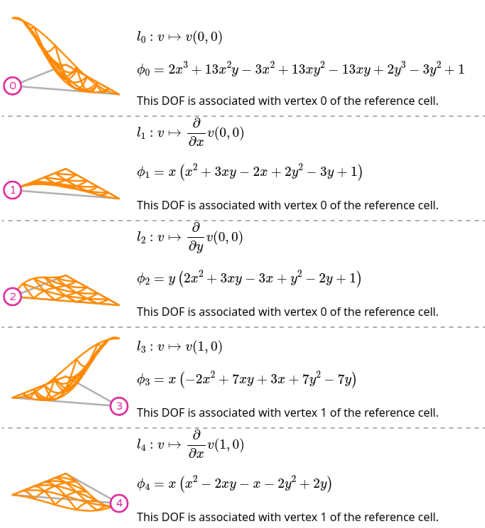
\includegraphics[width=\textwidth]{imgs/hermite_1.png}
        \end{subfigure}
        \begin{subfigure}[b]{0.4\textwidth}
            \centering
            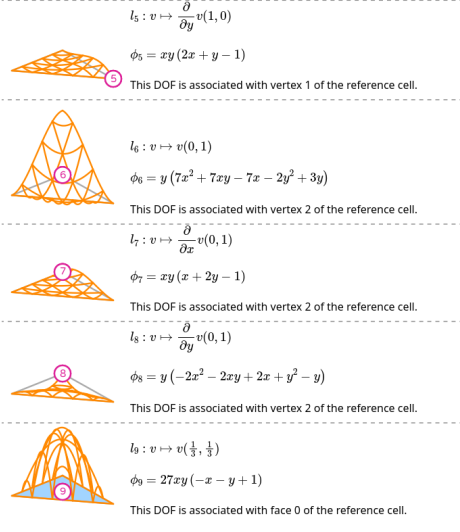
\includegraphics[width=\textwidth]{imgs/hermite_2.png}
        \end{subfigure}
        \caption{Basis functions of Hermite finite element}
    \end{figure}


    \begin{itemize}
        \item Degree 1 Taylor
    \end{itemize}
    Continuous across elements. 3 DoFs at the baricenter, two of them regarding the derivative.
    \begin{figure}[H]
        \centering
        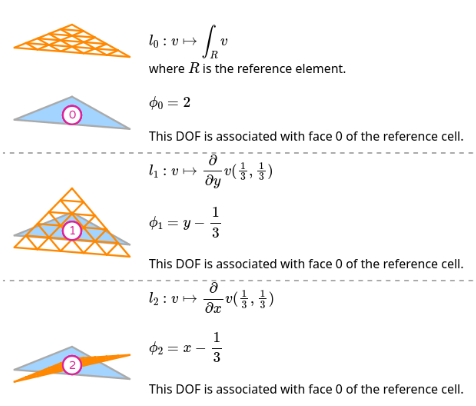
\includegraphics[width=0.7\textwidth]{imgs/taylor.png}
        \caption{Basis functions of Taylor finite element}
    \end{figure}


    \begin{itemize}
        \item Vector lagrange (Degree 1)
    \end{itemize}
    Describes vector functions ($f: \mathbb{R}^2 \to \mathbb{R}^2$). It's continuous across elements and uses 6 DoFs, 2 at each node.
    \begin{figure}[H]
        \centering
        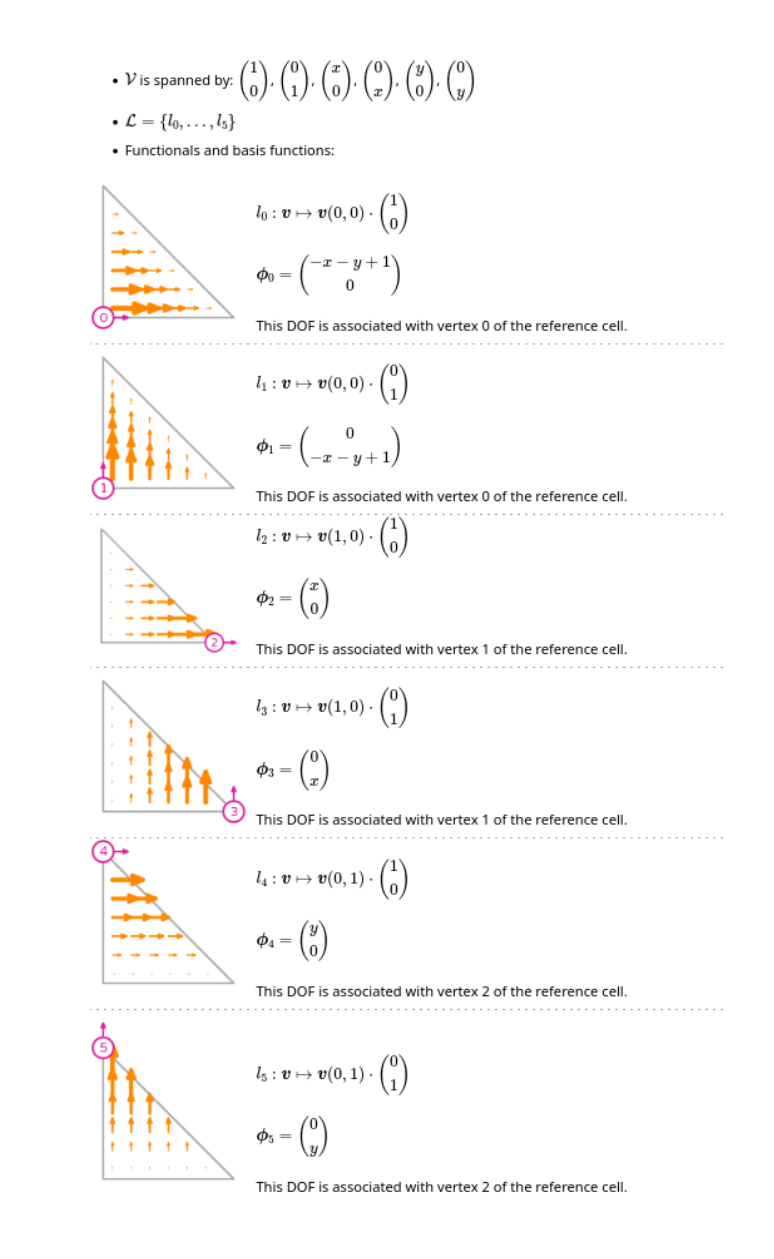
\includegraphics[width=0.7\textwidth]{imgs/vector_lagrange.png}
        \caption{Vector Lagrange basis functions}
    \end{figure}


    \begin{itemize}
        \item Crouzeix-Raviart
    \end{itemize}
    Discontinuous across elements. Uses 3 DoFs per element, 1 at the midpoint of each edge. At those points, there's continuity.
    \begin{figure}[H]
        \centering
        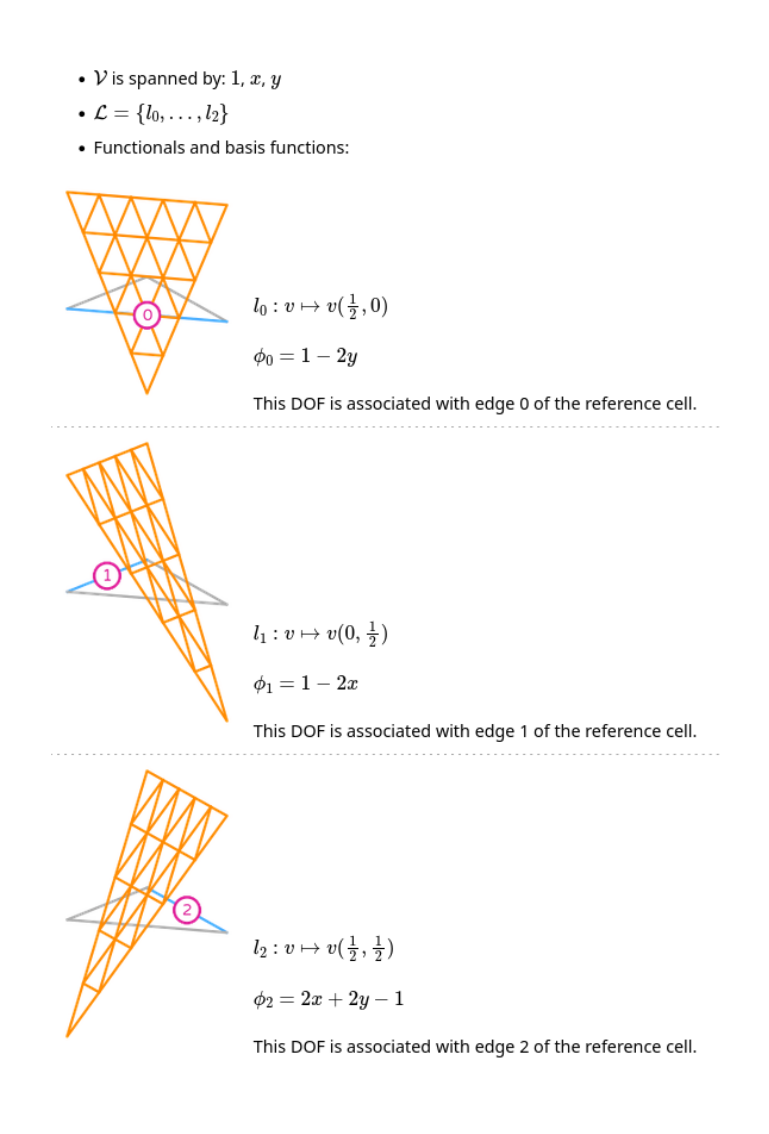
\includegraphics[width=0.8\textwidth]{imgs/crouzeix_raviart.png}
        \caption{Basis functions of Crouzeix-Raviart}
    \end{figure}


    \begin{itemize}
        \item Vector bubble enriched Lagrange (Degree 1)
    \end{itemize}

    Describes vector functions and is continuous across elements. Uses 8 DoFs: 2 for each node (1 for each direction) and 2 at the baricenter (1 for each direction).
    \begin{figure}[H]
        \centering
        \begin{subfigure}[b]{0.6\textwidth}
            \centering
            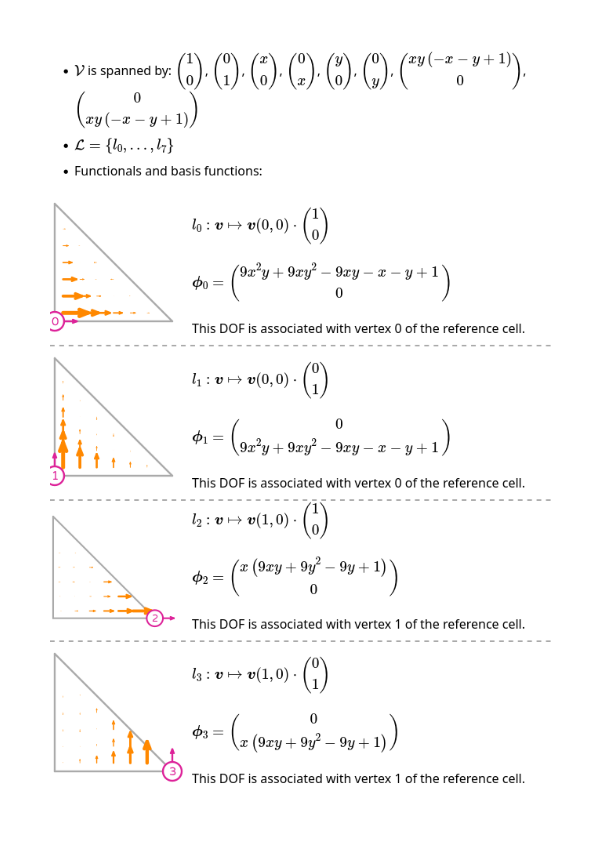
\includegraphics[width=\textwidth]{imgs/vector_bubble_enriched_lagrange_1.png}
        \end{subfigure}
        \begin{subfigure}[b]{0.6\textwidth}
            \centering
            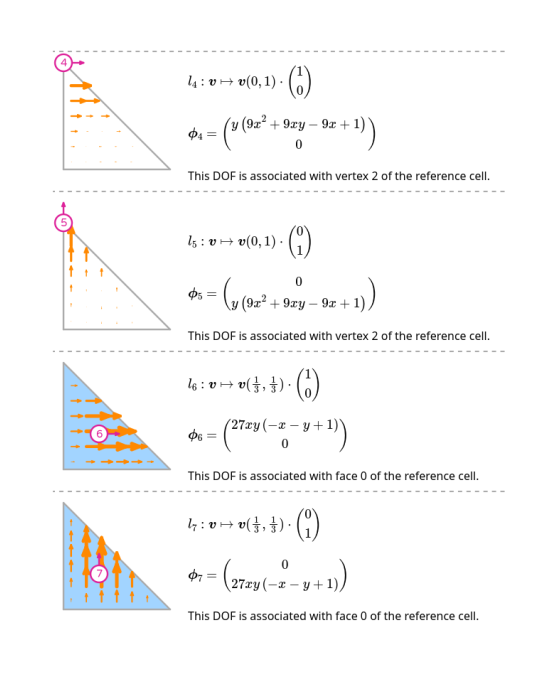
\includegraphics[width=\textwidth]{imgs/vector_bubble_enriched_lagrange_2.png}
        \end{subfigure}
        \caption{Basis functions of vector bubble enriched Lagrange}
    \end{figure}
\end{document}